\subsection{Visualizing Software Dependencies}

On Windows, there are many kinds of binary files.
We use the term program to denote the executable, which
is usually an EXE file in Windows.
Unlike Unix, Windows has many kinds of binary files containing
other software modules.
A non-comprehensive list of the binary files other than EXE
is as follows:
DLL (dynamic link libraries), ocx (ActiveX controls,
these are commonly used by Internet Explorer), sys (device
drivers, these may be in user or kernel mode), cpl (control panel applets),
acm/ax (multimedia codecs), etc.
In this section, we use the term EXE to denote the single main executable,
and the term DLL to denote binaries containing software other than the EXE.
We consider both EXE and DLL files used to be software modules.

The module dependencies are naturally visualized using a directed graph where
a directed edge from a node representing binary $A$ to another
node representing binary $B$ indicates that there is
a dependency, namely that code in $A$ makes use of code in $B$.
(We see later why there is the phrasing ``node representing a binary'' in
Sec. \ref{sec:exe-dep-graph}).
Given this classification of binaries, there are three possible
types of dependencies:
\begin{itemize}
\item {\bf EXE-DLL}: \\
This type of dependency represents the fact that a program uses a DLL.
For example, {\tt iexplore.exe} depends on {\tt mshtml.dll}.
\item {\bf DLL-DLL}: \\
DLLs can have dependencies among themselves.
For example, one of Mozilla's UI libraries {\tt xul.dll} depends on the SQLite
database library {\tt sqlite3.dll}.
\item {\bf EXE-EXE}: \\
Programs may also depend on other programs. This arises when a process
which is an instance of program $P_a$ creates another process
which is an instance of program $P_b$.
We also visualize this with an edge from $P_a$ to $P_b$ (thicker blue edge).
The label of an edge indicates the number of times $P_a$ creates $P_b$.
\end{itemize}

In this work, we are concerned with determining and visualizing these
dependencies at runtime, when the software (and there may be multiple
EXEs) run.
Instead of using a single visualization to show the three kinds of dependency
together, we propose two visualizations which are meant
to serve different purposes.
The first type of visualization, called EXE dependency graph,
shows the EXE-DLL and EXE-EXE dependencies.
The second type of visualization, called DLL dependency graph,
shows the EXE-DLL and DLL-DLL dependencies.
The EXE-DLL dependencies are different between the EXE dependency
graph and the DLL dependency graphs, i.e. they have different definitions
and visualizations.

\subsubsection{EXE Dependency Graph}
\label{sec:exe-dep-graph}

We first define what we mean by EXE-DLL and EXE-EXE dependency in
an {\em EXE Dependency Graph}.

\begin{definition}
An EXE-DLL dependency in an EXE dependency graph
is when process {\em a} running executable
$x$ loads binary $y$.
We say that $x$ has an EXE-DLL dependency on $y$.
\end{definition}
In Windows, a binary can be loaded explicitly by the {\tt LoadLibrary()} API,
or implicitly by the {\tt IMPORTS} file header.
Both of these lead to EXE-DLL dependencies.

\begin{definition}
An EXE-EXE dependency in an EXE dependency graph
is when process {\em a} running executable $x$ creates
a new process {\em b} which is running executable $y$.
We say that $x$ has an EXE-EXE dependency on $y$.
\end{definition}

EXE-EXE dependencies give a form of parent-child relationship.
However, is not the same as the process hierarchy graph
since the process hierarchy is about processes and the EXE-EXE
dependency is on files.
Furthermore, as we will see in the visualization,
there is only one node for every program and there can be cycles.

We are mostly concerned with dependencies between different executables,
hence, we omit self loops if there is an EXE-EXE dependency between $x$ and
itself.
We remark that in Windows, process creation is achieved in the WIN32 library
with the {\tt CreateProcess()} API (there
is an implicit dependency that {\tt kernel32.dll} relies on {\tt ntdll.dll}),
where\-as in Unix, a combination of the
{\tt fork()} and {\tt execve()} system calls
are used.

The EXE dependency graph visualization is motivated by scenarios when
we want to understand: (i) what various software modules have in common;
and (ii) where they are different.
Furthermore, a program may depend
on a number of other programs to do its work.

The EXE dependency graph has two kinds of nodes,
files which are EXEs, are denoted by ellipses, while
files which are DLLs, are denoted by rectangles.
(See Fig. \ref{fig:grouping}).
EXE-EXE and EXE-DLL dependencies are represented by
blue and black directed edges respectively.
In general, the EXE dependency graph forms a general graph rather than a
DAG since programs can mutually depend on one another
(this is a generalization of a call graph to the process level).

\begin{figure}
\centering
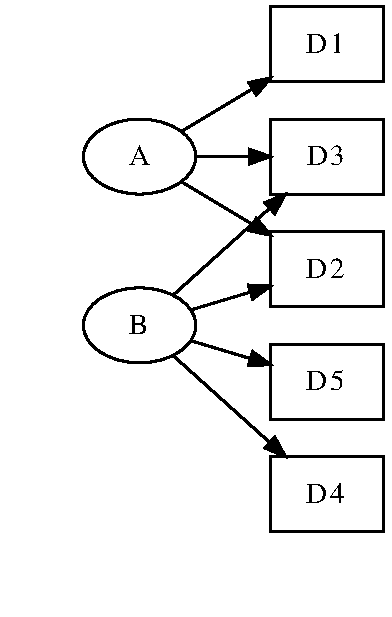
\includegraphics[scale=0.4]{depvis/example-split.pdf}
\hspace{15mm}
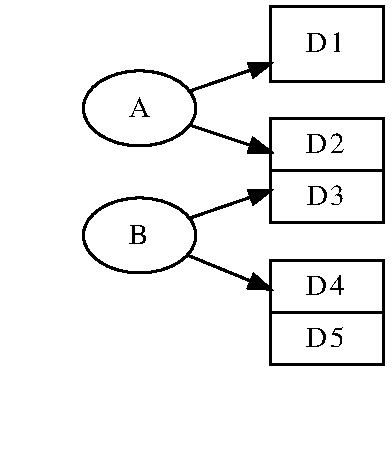
\includegraphics[scale=0.4]{depvis/example-group.pdf}
\caption{Dependency graph without (left) and with (right) grouping of programs
A and B with other DLLs D1 to D5}
\label{fig:grouping}
\end{figure}

In a direct visualization of EXE-EXE and EXE-DLL dependencies,
a directed edge between node $x$ and $y$ denotes that there is
the dependency between file $x$ and file $y$,
e.g. see the left graph in Fig. \ref{fig:grouping}.
This straightforward direct visualization is usually too complex
to be manageable as it often has too many nodes and edges simply
because there are many dependencies in Windows.
For example, in a fresh Windows install,
the {\tt C:/windows/system32} directory alone can contain more
than a thousand DLLs; while in a Windows system with more software installed,
there can be several thousand DLLs.
A simple program such as {\tt notepad.exe} loads more than 30 DLL files.

Thus, a more effective visualization is needed.
We propose a compressed dependency graph with fewer nodes.
This is obtained by grouping the DLL nodes according to the
EXEs which lead to that dependency,
i.e. incoming edges to the binary file.
More specifically, Let the set of all EXEs with a dependency on DLL $x$
be the program set of $x$.
We group all binaries whose program sets are the same.
Fig.~\ref{fig:grouping} shows the dependency graph without grouping (left) and
with grouping (right).

Since files often come from particular directories which are either system
directories or program directories and there are different binary types,
we further group files so that the files with the same directory and
same file type are in one node, e.g. label 4 in Fig. \ref{fig:browsers}
which shows the dependencies from DLLs which match with the
pathname {\tt /windows/system32/*.dll} (note that we have used
the forward `{\tt /}' for pathnames).

\paragraph{DLL Dependency Graph}

We define what we mean by EXE-DLL and DLL-DLL dependency in
a {\em DLL Dependency Graph}. The DLL dependency graph
is for a single process, so in the definitions below
we can assume that process $a$ is running executable $x$.

\begin{definition}
An EXE-DLL dependency in a DLL Dependency Graph
is when there is a control transfer from code in executable $x$
to code in DLL $y$.
We say that $x$ has an EXE-DLL dependency on $y$.
\end{definition}

\begin{definition}
A DLL-DLL dependency in a DLL Dependency Graph
is when there is a control transfer from code in
DLL $x$ to code in DLL $y$.
We say that $x$ has a DLL-DLL dependency on $y$.
\end{definition}

A DLL dependency graph shows how the code in DLLs depend
on each other. The motivation is that a DLL often has a certain functionality,
so the graph also illustrates the use of that functionality in an
abstract fashion. Furthermore, DLLs can depend on each other in a complex
fashion which is shown by this graph.
For example, DLL dependency graph can show how a DLL can have
a hidden dependency because it relies on other DLLs for certain functionality.

The DLL dependency graph shows module dependencies during execution
of a program.
In the graph, the nodes are either the single EXE or DLLs.
An edge from node $x$ to node $y$ represents a module or executable
in $x$ calling some code in module $y$.
We also call this as $x$ uses $y$.
Typically this means $x$ calls a function in $y$.
The label of an edge represents the number of invocations, i.e.
the number of calls from $x$ to $y$.
Note that it is possible for DLL $x$ to use DLL $y$ and also for
$y$ to use $x$ during the execution.
In this case, the edge between node $x$ and $y$ is bidirectional.
In the visualization, we use a thick line without any arrow.

A direct visualization of the DLL dependency graph is often too complex,
because there can be too many binaries used during an execution,
e.g. Fig \ref{fig:wget-nogroup} shows the graph for a small program {\tt wget}.
We use a simple idea that the visualization can be abstracted in two ways
by grouping.
One way of grouping is to group binaries which have a related function
in the same node, for example, we can group Windows DLLs which deal with
networking together.
Another way of grouping is to think of the source of the binary, so this
could be a way of grouping by software vendor.
For example, we can also group binaries which are from Adobe together.

The DLL dependency graph shows actual control flow dependency.
The EXE dependency graph, on the other hand, only shows what
DLLs are loaded. Obviously, in a DLL dependency graph,
if there is a path from executable $x$ to the node representing
DLL $y$ (due to grouping), then there will
be a direct edge in the EXE dependency graph between $x$ and the node
representing $y$ (due of grouping).
However, an edge in the EXE dependency graph does not imply that there is
such a path in the DLL dependency graph, simply because a DLL might
be loaded but not called.
It is useful to be able to tell that a DLL $y$ is not actually called,
although $y$ is loaded.
Such a DLL $y$ is labeled with the notation {\it *y*} in the DLL dependency
graph and are is not connected to any other nodes.

To further simplify the visualization, DLLs can have initialization code.
So control flow between EXE and DLLs due to initialization increases
the complexity of the graph. We allow for the visualization to ignore
dependencies which arise due to initialization which can reduce some
of the edges in the graph.
Note that this can lead to some nodes being disconnected from the graph,
and in some cases, those nodes will be treated as nodes which are not called,
i.e. labelled as {\it *y*}.
Our visualization can choose to either ignore DLL initialization or
to take it into account.

\subsubsection{Other DLL Dependency Graphs}

There are two DLL Dependency Graphs
which are obtained through {\em diff} and {\em projection} operations.

Sometimes we want to compare two executions of the same executable or
module.
For example, we want to identify which additional binaries are used when
we browse a web page with Adobe Flash versus browsing without Flash.
We can then conjecture that those additional binaries are related to the
Flash component.
We also want to know which additional module invocations/dependencies
are incurred by Flash.
To visualize this,
it is useful to define the graph difference between the two graphs,
which we call {\em diff}.
The diff of graph $A$ and $B$, denoted by $A-B$,
is essentially subtracting graph $B$ from $A$.
The result is that only edges that appear in $A$ but not in $B$ appear
in the resulting {\em diff} graph.
A DLL $x$ which only appears in $A$ but not in $B$ is annotated
as {\it +x+}.

Sometimes we want to focus on a specific binary - or a group of binaries.
For example, we want to know which binaries are used by the cryptography
library {\tt crypt32.dll}, and correspondingly,
which binaries use {\tt crypt32.dll}.
We want to determine not only which binaries are directly used,
but also those which are indirectly used.
We propose the {\em projected} DLL dependency graph for this purpose.
In the graph projected on a set of binaries $S$,
only binaries that are used by $S$ or binaries that use $S$ either directly
or indirectly are shown.
Note that this is not the same as finding connected components containing
$S$ in the dependency graph.
This is because the dependency graph loses some information.
Instead, the projection looks at the control flow chain during
execution and selects all the DLLs which have $S$ in its path.
Since projection removes edges from the original graph, we have the
option to keep DLLs which are not in the projection but are used
(this makes sense under grouping) and we label the node as {\it \#y\#}

\begin{figure}
\begin{minipage}[t]{3.5cm}
\begin{verbatim}
void main (void) {
   A();
   B(1);
}
void C (void) {}
void D (void) {}
\end{verbatim}
\end{minipage}
\hspace{1.0cm}
\begin{minipage}[t]{3.0cm}
\begin{verbatim}
void A (void) {
   B(0);
}
void B (int i) {
   if (i) D();
   else C();
}
\end{verbatim}
\end{minipage}
\caption{Each function is its own DLL}
\label{fig:indcalls}
\end{figure}

The following example illustrates why the difference between
projection and connected components in the graph.
The program in Fig.~\ref{fig:indcalls} has
five functions which are in DLL modules of the same name.
Suppose we project on {\tt A.dll}.
Only {\tt main.exe} uses {\tt A.dll} directly.
{\tt A.dll} uses {\tt B.dll} (directly) and
{\tt C.dll} (indirectly).
{\tt D.dll} is used by {\tt B.dll} but never by {\tt A.dll} at runtime.
Thus, the projection on {\tt A.dll} does not contain {\tt D.dll} even though
it is reachable from {\tt A.dll} in the DLL dependency graph.

